\documentclass[10pt,a4paper]{report}
\usepackage[utf8]{inputenc}
\usepackage{amsmath}
\usepackage{amsfonts}
\usepackage{amssymb}
\usepackage{stackengine}
\usepackage{hyperref}
\usepackage{wrapfig}
\usepackage{graphicx}
\author{Aaron Lau}
\title{The Search for the Hidden Valley}
\begin{document}

\part*{The Search for the Hidden Valley}
%BODY
\section*{Introduction}

"The Search for the Hidden Valley" is a search for theoretical dark matter particles. Specifically, we are looking for Hidden Valley Pions ($\pi_s$). When a Higgs boson($H$) decays, it can decay a few different ways. It is hypothesized that one of the possibilities is a pair of Hidden Valley Pions.\\\\
In order to test this hypothesis, we need to cause many thousands of particle collisions at a real particle accelerator. Since a Higgs boson only has a chance to decay into the Hidden Valley Pions, only a small fraction of  these collisions are expected to be Hidden Valley decays. Due to the large scale of this operation, it is unreasonable to manually watch every event and analyze it to see if it is a Hidden Valley decay. We must find an easier way to process such a large amount of data.\\\\
Our solution is to train a neural network to recognize the Hidden Valley decays for us. Neural networks are trained to recognize patterns. By looking at many examples of that same pattern, it learns what the defining features are. In this case, we want to teach our neural network what a Hidden Valley decay is supposed to look like by using simulations and then get it to find that pattern in real data.

\section*{Once More, with Physics}
\begin{wrapfigure}{L}{0.4\textwidth}
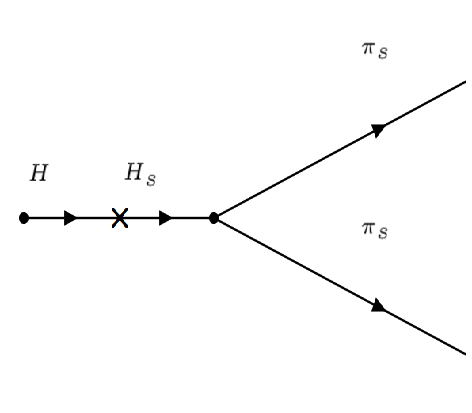
\includegraphics[scale=.4]{Figure1}
\begin{center}
{\scriptsize Figure 1: Hidden Valley Decay of a Higgs Boson}
\end{center}
\end{wrapfigure}

A Higgs boson has a rest mass of 125 GeV and is predicted to exist in a superposition of states. There is the standard model state, and the hidden valley state. When the $H$ decays from the hidden valley state, it decays into two $\pi_s$. The rest masses of the two $\pi_s$ are unknown to a certain extent. Since each $\pi_s$ decays into two b-quarks each with rest mass 5 GeV, the $\pi_s$ rest mass must be greater than 10 GeV. The sum of the two $\pi_s$ rest masses must also not exceed 125 GeV. A Feynman diagram (Figure[1]) is used to show the process of the Hidden Valley decay.\\\\
%In this paragraph, I will talk about the physical properties of the Hidden Valley decay. Higgs 125 GeV. b-quark 5 GeV. $\pi_s$ have unknown (tunable) rest masses try 30 GeV. We THINK they are long lived.  (This includes the rest masses of $H$ and $\pi_s$ as well as relativistic speeds, lifetimes (lab and rest frame), and a Feynman diagram for Figure[1]. LaTeX package Feynman diagram, TecZ Feynman.
%\begin{center}
%$\tau = \textit{I}\alpha$\\{\scriptsize Equation 1}
%\end{center}\\
%THIS IS AN EXAMPLE OF AN EQUATION
To simulate these Hidden Valley decays, we are using an ATLAS software distribution. ATLAS is the detector connected to the Large Hadron Collider at CERN. The name ATLAS is given to the programs, people, and everything associated with the operation of the detector.\\\\
The software creates simulations whose data can be stored in just one file called an event file. By [Creating an Event File], we are recording physical properties associated with each particle (such as velocity). We will look at some of these data later.\\\\
The simulations used to create the event file are modified slightly from their original form. Within the default programming (and in real life), there is only a small chance that the Higgs boson will decay into two $\pi_s$. This means that only a small fraction of our events would be $\pi_s$ decays. Since we are only interested in training the neural network to recognize the $\pi_s$ decays, we can override the probability and set it to 100\%. Now, a Higgs boson will always decay into two $\pi_s$. This has the same effect as filtering out all of the non-$\pi_s$ decays but with much less wasted effort.\\\\

\begin{wrapfigure}{L}{0.5\textwidth}
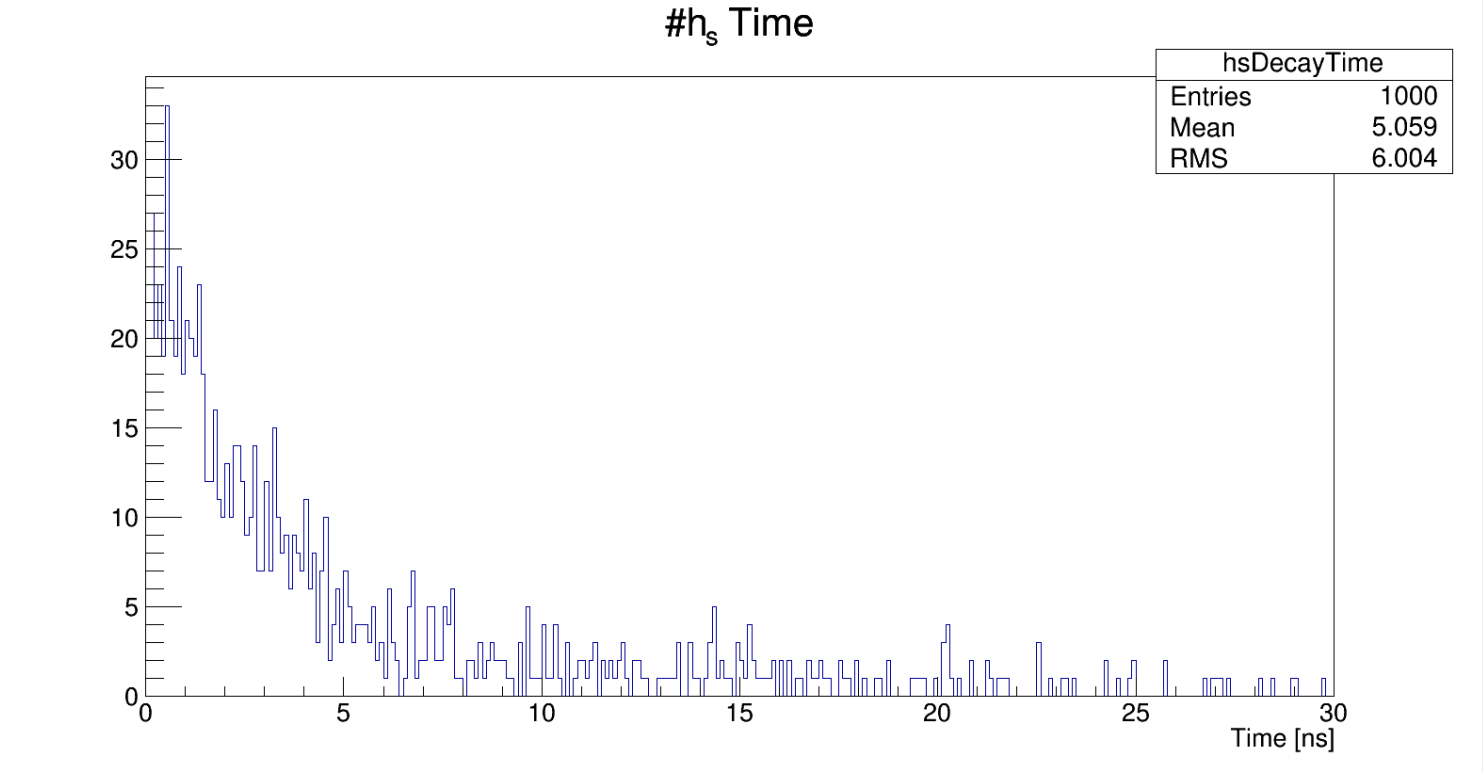
\includegraphics[scale=.16]{Figure2}
\begin{center}
{\scriptsize Figure 2: Distribution of $\pi_s$ lifetime in the lab frame}
\end{center}
\end{wrapfigure}

\noindent Having the event file is one step closer to training the neural network, but we need to make sure it is a good event file. It is necessary to manually check the event file to make sure that the data was generated properly. By [Making Histograms], we can see the distributions of various data contained within the file. Figure[2] is an example of a histogram, it shows the distribution of the lifetimes of the $\pi_s$ (shown as $\#h_s$ on the graph).\\\\
To make sure that an event file was generated properly, the histograms must have sensible data. For example, there should never be any particles with negative speed, and the lifetimes of the particles should be appropriate for the type of particle. Ultimately, the goal is to ensure that the distribution of data makes sense, and what makes sense could vary over different experiments.

\begin{wrapfigure}{L}{0.45\textwidth}
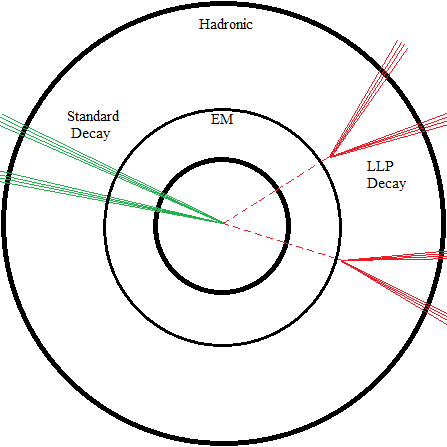
\includegraphics[scale=.4]{Figure3}
\begin{center}
{\scriptsize Figure 3: Standard decay vs a Long Lived Particle decay in detector}
\end{center}
\end{wrapfigure}

\noindent \\There are a few variables contained in the event file that we want to look at specifically. Namely CalRatio, JetPT, and TrackCount. CalRatio is defined as $log_{10}(\dfrac{E_H}{E_{EM}})$, which is the logarithmic ratio of energy absorbed by the Hadronic detector to the energy absorbed by the Electromagnetic detector. JetPT is defined as the net momentum of a Jet. TrackCount is the number of Tracks that spray out from one Jet. Figure[3] shows the process of a Hidden Valley decay in the ATLAS detector.\\\\
It is expected that $\pi_s$ are long lived particles. We expect $\pi_s$ to travel quite a bit before decaying, putting them further from the center of the detector. Due to this displacement, the CalRatio for Hidden Valley decays is likely to be much greater than zero. The $\pi_s$ decays also have just as easily distinguished values for JetPT and TrackCount, although in a different context. Using these three variables, we can create a pattern on which train a neural network.\\\\
We can now begin [Training a Neural Network]. Training involves ... This paragraph will be about putting the event file to work. Needs discussion, I know little

\section*{Creating an Event File}
Creating an event file is the first step in the process. So Here is where I go very in depth about creating an event file. Gritty stuff, stuff like screenshots of the terminal. Basically a functional tutorial on how to get from nothing to event file. Covers the time period from ~2 quarters ago
\section*{Making Histograms}

\begin{wrapfigure}{L}{0.5\textwidth}
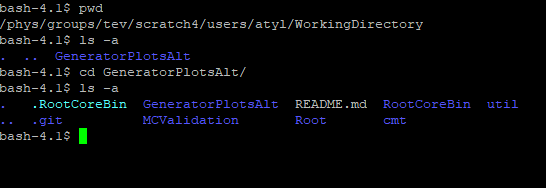
\includegraphics[scale=.4]{Figure4}
\begin{center}
{\scriptsize Figure 4: Cloning the Repository}
\end{center}
\end{wrapfigure}

Our histograms are contained within a root file. Root is a framework used by ATLAS that is very efficient at storing large amounts of data and accessing it quickly. The process of making a histogram-containing root file starts with having an event file.\\\\
To create this root file, it involves some coding. At this point, the C++ files required to create a Root file already exist and are working. They are pretty complicated, so this section will explain how to obtain and use them without much modification.\\\\
The first step is to visit GitHub. The current repository is located \href{https://github.com/AtlasWHHV/GeneratorPlotsAlt}{\underline{here}}. Create a working directory and clone this repository. After the clone is complete, the directories should appear similar to Figure[4].\\\\
In the 'util' folder, there should be a C++ file named PlotGeneratorQuantities.cxx. Among other things, this file finds the event file. Lines 51-52 of PlotGeneratorQuantities.cxx contain a system variable called \$DATAPATH. \$DATAPATH determines where PlotGeneratorQuantities.cxx searches for the event file, so make sure that it always points to the right place. \$DATAPATH can be set from the terminal using the command \verb|'export DATAPATH=/this/is/a/data.path'|\\\\
Now that the \$DATAPATH points to the right place, we can compile the program. From the working directory, the following commands must be executed in order:

$\cdot$\verb|${ATLAS_LOCAL_ROOT_BASE}/user/atlasLocalSetup.sh|

$\cdot$\verb|lsetup 'rcSetup Base,2.4.14'|

$\cdot$\verb|rc find_packages|

$\cdot$\verb|rc compile|\\
It takes a few minutes.\\\\
Once it is done compiling, we just need to run the program. If it compiled successfully, we should be able to just type \verb|PlotGeneratorQuantities| into the terminal. If this command executes successfully, there will be a new folder in the working directory called \verb|submitDir|. The root file is in \verb|submitDir|.\\\\
To open the root file, it is easiest to use a program called VNC Viewer. Download this online. Opening VNC Viewer shows an entry field a VNC Server address, so let's start the VNC Server. In the standard terminal, enter the command \verb|vncserver -geometry 1920x1080 :2|, it will ask for your password twice. Once this is complete, use VNC Viewer to connect to the server address displayed in the terminal. It should look similar to \verb|tev05.phys.washington.edu:2|. VNC Viewer looks like a Linux based desktop. You can even open a terminal within the VNC Viewer. Using this VNC Terminal, execute the following terminal commands (must be in Bash):

$\cdot$\verb|root -l|, this starts root

$\cdot$\verb|new TBrowser|\\\\
Then browse for the root file! The process should appear similar to Figure[5]

\begin{wrapfigure}{L}{0.5\textwidth}
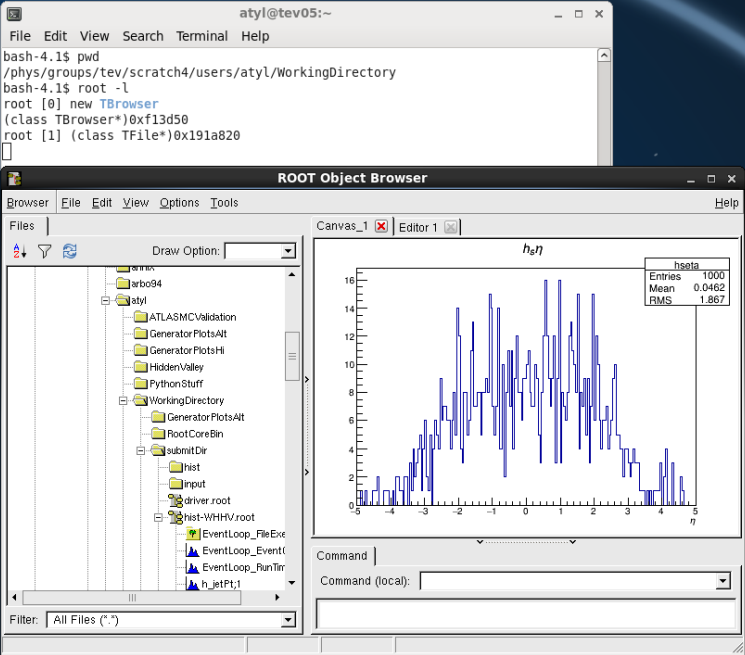
\includegraphics[scale=.3]{Figure5}
\begin{center}
{\scriptsize Figure 5: Using VNC Viewer}
\end{center}
\end{wrapfigure}
\noindent \\The reason we must use VNC Viewer is because the terminal we normally use does not have a display set up. In order to actually see the histograms in the ROOT file, we need such a display. The VNC Viewer has this display set up by default, so it is easy to open the ROOT file from the VNC Terminal.\\\\\\\\\\\\\\\\

\section*{Training a Neural Network}

\part*{Tools of the Trade}
\section*{GitHub}
GitHub is a platform hosted online that helps multiple people work together on the same project. The location of all of the project's files and assets is called a repository. Users can clone the online repository onto their local device, modify the files, and merge them back into the online repository.\\\\
GitHub automates the merging process by checking for differences between the online version and the newly modified local version, and updating the online repository accordingly. This removes the need to completely re-upload every file every time there is a small change.\\\\
Each GitHub repository can have multiple branches. There is always one branch called \verb|master|. The purpose of the branches is support the testing of different versions of the same project. Convention has that the \verb|master| branch should always be stable, meaning it compiles and executes with no modification. Later on, it is necessary to find out what branch is currently being worked on, or make your own.\\\\
The very first step to using GitHub is to register an account online. There will be authentication passwords that need to be created along the way, these will come up again later. The rest of this section will have the assumption that a GitHub account is already created, and access to the desired repository has already been granted by its administrator.\\\\
To begin working on a project, it is necessary to clone the repository. This can easily be done through the terminal by using the command\\ \verb|git clone bttps://github.com/AtlasWHHV/GeneratorPlotsAlt|,\\ the URL will of course change depending on the repository.\\\\
Now that the repository is cloned onto a local machine, it is time to make any changes or developments. The status of the local version compared to the online version can be checked with \verb|git status|. The default branch that gets modified is \verb|master|, so it is necessary to change to a different branch. The \verb|master| branch should never be modified directly. Switch branches using \verb|git checkout branchname|.\\\\
Once the desired changes are made, it is time to merge all of the changes into the online version. First, check the status by using \verb|git status|, then use the following terminal commands in order:

$\cdot$\verb|git add -a|

$\cdot$\verb|git commit -m "This is a description of the changes"|

$\cdot$\verb|git push|\\


\section*{Terminal}
The terminal is where most of the work on this project will be done. There are a few ways to open a terminal, here is one option. Download PuTTY online. In the \verb|host name| field, enter \verb|tev04.phys.washington.edu| and connect. Nothing else needs to be modified. It should open up a terminal asking for your login information.\\\\
The terminal is functional on its own, but more specifically we use Bash. Bash is a type of Unix shell. To begin using Bash, type \verb|bash| into the command line and then select option 1 to use Root version 5.34.\\\\
There are a many terminal commands that are not unique to Bash. These are mostly for navigating and manipulating files and directories. A few of the most critical ones are listed here:

$\cdot$\verb|pwd|, displays the current directory.

$\cdot$\verb|ls|, lists the contents of the current directory.

$\cdot$\verb|cd /this/is/a/directory|, changes the directory

$\cdot$\verb|help|, displays a list of terminal commands and a brief description of their function.

$\cdot$\verb|man|, putting \verb|man| before any other command will bring up a detailed manual about that function, \verb|man pwd| for example.\\
There are \textbf{many} more terminal commands than exist on this list, many of which are incredibly useful.\\\\
When using Bash, almost anything can become a terminal command using Aliases. An Alias is usually a shorter string that conveniently represents a much larger string. For example, I could use the string \verb|lset| as a shortcut to the longer command \verb|lsetup 'rcSetup Base,2.4.14'|. Aliases are very useful to avoid tedious commands, especially in the case of navigating to a specific directory.
\section*{Vim} 
Vim is a text editor that is built into the terminal. Using the command \verb|vim filename.extension| will open that document in Vim. Once opened, Vim has a command line that appears once you type a colon (\verb|:|). Here are a few of the basic commands:

\verb|:q|, Quits Vim, will not work if there are unsaved changes made to the document.

\verb|:wq|, Saves (writes) the changes made to the document and then quits Vim.

\verb|:w|, Only saves the changes made to the document.

\verb|:q!|, Force quits Vim and discards all changes.\\\\
To navigate around the document, use the arrow keys. The cursor will move one character at a time. Now it is possible to modify the document:

\verb|r|, typing \verb|r| while there are no other characters in the command line will enter replace mode. The next character you type will replace the character highlighted by the cursor.

\verb|i|, Enters Insert mode. This is basically a normal text editor mode that allows larger modification of the document.

\end{document}
